\chapter{Combinatorics}\labelandindex{Combinatorics}


\section{Permutation} \labelandindex{Permutations}
The permutation of a set can be defined as an arrangement of the members of the set; or the act of creating or changing such an arrangement. Common examples are Anagrams, which consist of different ways of arranging letters in a word.

\begin{equation}
    \Perm{n}{r} = \frac{n!}{(n-k)!}
\end{equation}

\subsection{Basic Permutations}

\begin{table}[h]
    \renewcommand{\arraystretch}{1.5}
    \centering
    \begin{tabularx}{\textwidth}{Xc}
        \toprule
        \textbf{Description}                                                                                                                                                                                                            & \textbf{Formula}                              \\
        \midrule
        No. of arrangements of \mbox{$k$} distinct objects out of \mbox{$n$} total objects without repetition                                                                                                                           & \mbox{$\Perm{n}{r}$}                          \\
        No. of arrangements of \mbox{$k$} distinct objects out of \mbox{$n$} total objects \textbf{with repetition}                                                                                                                     & \mbox{$n^k$}                                  \\
        \marginnote{Assuming \mbox{$k$} sets each having a certain number of repetitions with \mbox{$n_k$} items}No. of arrangements of \mbox{$k$} distinct objects out of \mbox{$n$} total objects \textbf{with restricted repetition} & \mbox{$\frac{{n!}}{n_1!\;n_2!\;\dots\;n_k!}$} \\
        Circular permutation where direction is important                                                                                                                                                                               & \mbox{$(n-1)!$}                               \\
        Circular permutation where direction is \textbf{not important}                                                                                                                                                                  & \mbox{$\frac{(n-1)!}{2}$}                     \\
        \bottomrule
    \end{tabularx}
    \caption{Basic Permutation Formulae}
    \label{tab:basic_Permutations}
\end{table}

\section{Combination}

\begin{align}
    \Comb{n}{k}\times k! & = \Perm{n}{k} \nonumber            \\
    \Comb{n}{k}          & = \frac{\Perm{n}{k}}{k!} \nonumber \\
    \Comb{n}{k}          & = \frac{n!}{k!\;(n-k)!}
\end{align}

Alternatively, \mbox{$\Comb{n}{k}$} can be considered in terms of binomial coefficient \mbox{$\begin{pmatrix} n \\ k\end{pmatrix}$}. In that case, by using the binomial expansion formula, we can derive \mbox{$\Comb{n}{k}$}. The formula for a binomial coefficient is
\begin{align}
    \begin{pmatrix} n \\ k\end{pmatrix} & = \frac{n\times (n-1) \times (n-2) \dots \times (n-k+1)}{k\times (k-1) \times (k-2) \dots \times 1} \nonumber
\end{align}
We can multiply the fraction with \mbox{$(n-k)!$}, which allows us to write
\begin{align}
    \begin{pmatrix}
        n \\
        k
    \end{pmatrix}
     & = \frac{\overbrace{n\times (n-1) \times (n-2) \dots \times (n-k+1)\times \overbrace{(n-k) \times (n-k-1) \dots \times 1}^{(n-k)!}}^{n!}}{\underbrace{k\times (k-1) \times (k-2) \dots \times 1}_{k!}\times \underbrace{(n-k) \times (n-k-1) \dots \times 1}_{(n-k)!}} \nonumber
\end{align}
and we can simplify to
\begin{align}
    \begin{pmatrix} n \\ k\end{pmatrix} = \frac{n!}{k!\times (n-k)!} = \Comb{n}{k}
\end{align}

\subsection{Symmetry of Combinations}
Combinations inherently have a symmetric property. Suppose you have a set of five objects, out of which two need to be selected. This is equivalent to the case where you select three objects to leave behind. Formulaically, we can derive the relation as
\begin{align}
    \begin{pmatrix}
        n \\k
    \end{pmatrix} & = \frac{n!}{k!\times (n-k)!} \nonumber
\end{align}
now substitute the case where \mbox{$k=n-k \Rightarrow 2k = n \Rightarrow k = \frac{n}{2}$}
\begin{align}
    \begin{pmatrix}
        n \\k
    \end{pmatrix}                                                                                                                                  & = \frac{n!}{(n-k)!\times (n-(n-k))!} \nonumber              \\
    \begin{pmatrix} \marginnote{This happens because there are factors which are common to both the denominator and numerator and get canceled out.}
        n \\k
    \end{pmatrix} & = \frac{n!}{(n-k)!\times (\cancel{n-n+}k)!} \nonumber                                                              \\
    \begin{pmatrix}
        n \\k
    \end{pmatrix}                                                                                                                                  & = \frac{n!}{(n-k)!\times k!} =     \begin{pmatrix}
                                                                                                                                                                                            n \\n-k
                                                                                                                                                                                        \end{pmatrix}\nonumber \
\end{align}

\subsection{Basic Combinations}
Table \ref{tab:basic_combinations} gives a list of basic combination formulae. The number of combination formulae is significantly less than permutation formulae as order is irrelevant for this case.
\begin{table}[h]
    \renewcommand{\arraystretch}{1.5}
    \centering
    \begin{tabularx}{\textwidth}{Xc}
        \toprule
        \textbf{Description}                 & \textbf{Formula}         \\
        \midrule
        Combination without repetition       & \mbox{$\Comb{n}{k}$}     \\
        Combination \textbf{with repetition} & \mbox{$\Comb{n+k-1}{k}$} \\
        \bottomrule
    \end{tabularx}
    \caption{Basic Combination Formulae}
    \label{tab:basic_combinations}
\end{table}

\section{Distributions}\labelandindex{Distributions}
\Tree [ .Distribution [ .Distinct\ Objects\\(Permutation) ] [ .Identical\ Objects\\(Combination) ] ]
\Tree [ .Distribution [ .\text{Any number of objects per box}\\(Repetition) ] [ .\text{At most one obj per box}\\(No\ Repetition) ] ]
\begin{exampletcb}
    {Finding Roots of an Equation}{}
    Find the total number of non-negative solutions to \mbox{$x_1+x_2+x_3+x_4+x_5+x_6 = 4$}.

    \textbf{Ans:} First, we start by taking random solutions. By trial and error we can see that \mbox{$(1,0,1,1,0,1)$} and \mbox{$(4,0,0,0,0,0)$} are solutions. Now we can see that this is a problem for distributions. We have to distribute 4 `1's into 6 places, and we can have any number of `1's in each box. i.e. identical objects (combination) and any number of objects per box (repetition). So, we use the formula \mbox{$\Comb{n+r-1}{r}$}, with \mbox{$r = 4$} \mbox{$n = 6$}.
    \[
        \Comb{6+4-1}{4} = \Comb{9}{4} \text{ ways.}
    \]
\end{exampletcb}

\begin{exampletcb}
    {Scheduling Exams}{}
    Find the number of ways in which 3 exams can be schedules in 5 days such that \\
    \begin{enumerate}
        \item No two exams are on the same day.
        \item No restrictions on the number of exams per day.
    \end{enumerate}

    \textbf{Ans:} This is a very typical distribution question. It consists of distint objects, so it is a permutation. We can also see that the subquestions are based on a case with repetition and a case without repetition.
    \begin{enumerate}
        \item \mbox{$\Perm{5}{3}$}
        \item \mbox{$5^3$}
    \end{enumerate}
\end{exampletcb}



\begin{exampletcb}
    {Odd Numbers With Distint Digits}{}
    How many odd integers exist between 100 and 999 and have distinct digits?

    \textbf{Ans:} This is a little trickier to answer. It is not clear as to which category this question belongs to. So we will take the normal route and try to come to an answer. First we list out all the restrictions that we need to adhere to.
    \begin{itemize}
        \item Three digit number - no 0 in the first box.\marginnote{Here, we have an example of a situation with multiple restrictions. In such cases, we deal with the digit or position with the most restrictions.}
        \item Odd number - restricted third box to odd numbers only.
        \item Distinct digits - all boxes.
    \end{itemize}
    Now, we start building out number based on these restrictions. We will take the last box, since it has the most restriction (0, 2, 4, 6, 8 cannot take that place). The numbers here represent the number of choices for a particular position.
    \[
        \boxed{}\boxed{}\boxed{5}
    \]
    Then we move on to the next most restrictied position, position 1. Here, we cannot use a 0 and the number used in the last box, that leaves us with 8 choices.
    \[
        \boxed{8}\boxed{}\boxed{5}
    \]
    Finally we come to the box with the least number of restrictions, box 2, which has to have digits not already used in box 1 and 3. \marginnote{In continuation of the previous note, suppose we filled 0 in the second box. In that case, we would not need the 0 restriction in the first box.}
    \begin{align*}
         & \boxed{8}\boxed{8}\boxed{5}      \\
         & 8 \times 8 \times 5 \text{ ways}
    \end{align*}
\end{exampletcb}


\begin{exampletcb}
    {Number of Integers With Distinct Digits}{}
    How many of the first 1000 integers have distinct digits?

    \textbf{Ans:} This is a classic example of a multi-case question. In multi-case questions, there will not be any possible generalisation that you can apply to all the objects in question, in this instance, to numbers. So, we consider three cases. One digit, Two digit, and three digit. The specifics of arriving to the answer is left to the reader as an exercise.
    \begin{itemize}
        \item One digit: \mbox{$\boxed{9}$} ways.
        \item Two digits: \mbox{$\boxed{9}\boxed{9}$} ways. \marginnote{Why is it (9,9) and not (9,8)?}
        \item Three digits: \mbox{$\boxed{9}\boxed{9}\boxed{8}$} ways.
    \end{itemize}
\end{exampletcb}


\begin{exampletcb}
    {Selecting Integers to Sum To a Multiple of 3}{}
    In how many ways can we select 3 integers from \mbox{$3n$} consecutive integers such that their sum is a multiple of 3?

    \textbf{Ans:} Admittedly, this is a tricky question. It would be advantageous to first understand what is being asked here. The question takes a set of consecutive integers, from 1 to \mbox{$3n$}, with n being an arbitrary natural number. Then, we have to count the number of subsets, containing three elements, that sum up to a multiple of three. In such cases, we first have to identify any possible simplifications in the question.

    We can see that the set of integers from 1 to \mbox{$3n$}, can be split into three sets each of which has \mbox{$\frac{3n}{3} = n$} elements,
    \begin{align*}
        x\%3 ==0 & \rightarrow\;0,3,6\dots3n\marginnote{It would be warranted to think that the last element of this series should be \mbox{$3n+2$}, but we have to note that \mbox{$3n+2>3n$} and so \mbox{$3n+2-3$} would give the previous (and last) element in the series.} \\
        x\%3 ==1 & \rightarrow\;1,4,7\dots3n-1                                                                                                                                                                                                                                   \\
        x\%3 ==2 & \rightarrow\;2,5,8\dots3n-2                                                                                                                                                                                                                                   \\
    \end{align*}
    Now, we can simplify the question. We not that we can choose any three numbers from the group \mbox{$3n$} and we would still get a subset divisible by three. Similarly, we can choose three numbers from the other two groups and get the same result. Additionally, we can select one number from \mbox{$3n$},\mbox{$3n-2$} and \mbox{$3n-1$} to give \[
        \sum\left\{3n, 3n-1, 3n-2\right\} = 3\times 3n - 3
    \] which is still divisible by three. We have to repeat the same procedure to identify any other combinations that fit our question, which is none in this case.
    Finally, we sum up all these combinations to get our answer.
    \[
        \underbrace{\Comb{n}{3}}_{3n} +\underbrace{\Comb{n}{3}}_{3n-1} + \underbrace{\Comb{n}{3}}_{3n-2} + \underbrace{\Comb{n}{1}\Comb{n}{1}\Comb{n}{1}}_{\text{one from each}} \text{ways}
    \]
\end{exampletcb}


\begin{exampletcb}
    {Permutations of INSTITUTION}{}
    Find the number of permutations of the word INSTITUTION.
    \begin{itemize}
        \item Find the number of them that begin with I and end with N.
        \item How many permutations are possbile if three Ts should not be together?
    \end{itemize}

    \textbf{Ans:} This is a straight-forward question. The total number of permuations of \mbox{$n$} objects, with partial repetition is given in table \ref{tab:basic_Permutations}. Comparing with the formula, we see that there are 11 letters (\mbox{$n=11$}), with 3 Is and Ts (\mbox{$n_1=3, n_2=3$}). So, the total number of permutations will be
    \[
        \frac{11!}{3!\times 3!\times 2!}
    \]
    Next, we move onto the subquestions. For the first one, we fix I and N in their respective places. So,
    \[
        \boxed{I}\boxed{}\boxed{}\boxed{}\boxed{}\boxed{}\boxed{}\boxed{}\boxed{}\boxed{}\boxed{N}
    \] Basically simplifying the permutation to 9 objects. So the answer to the second part is
    \[
        \frac{9!}{2! \times 3!}
    \]
    For the third part, we need to find the total number of permutations which are having 3 Ts together. Consider these three Ts as one object, alongside the other letters. Now, we can find the total number of permutations in this case.
    \[
        \frac{9!}{3!\times 2!}
    \]
    Now finding the complement,
    \begin{align*}
        \left\{\text{All possible permutations}\right\} & - \left\{\text{All possible permutations with TTT}\right\}             \\&= \left\{\text{All possible permutations without TTT}\right\} \\
                                                        & \frac{11!}{3!\times 3!\times 2!} - \frac{9!}{3!\times 2!} \text{ ways}
    \end{align*}
\end{exampletcb}


\begin{exampletcb}
    {A New National Flag}{}
    A new national flag needs to be designed with blue, green, yellow and red. It has 6 strips. In how many ways can we colour the strips such that no two adjacent strips have the same colour?

    \textbf{Ans:} This is easy. For the first strip, we can choose one out of 4 colours. For the next strip, we choose one of 3, as one colour is already taken by the previous strip. Similarly, we have 3 choices for the third strip (not 2 choices) and so on.
    \[
        4\times3\times3\times3\times3\times3\text{ ways}
    \]
\end{exampletcb}


\begin{exampletcb}
    {Choosing Days of a Week}{}
    In how many ways can you choose three days out of a week with repetition allowed?

    \textbf{Ans:} \mbox{$n=7,r=3;\quad \Comb{7+3-1}{3} = \Comb{9}{3}\ ways$}
\end{exampletcb}

\begin{exampletcb}
    {Sum of Permutations}{}
    Find the sum of all 4 digit numbers that can be obtained by using the digits 1, 2, 3, 4 once in each.

    \textbf{Ans:} The answer to this may not be obvious at first. So, we try permuting these numbers. We already know that there will be \mbox{$4!$} permutations, from this set
    \[
        \begin{Bmatrix}
            1      & 2      & 3      & 4      \\
            1      & 2      & 4      & 3      \\
            1      & 4      & 2      & 3      \\
            \vdots & \vdots & \vdots & \vdots
        \end{Bmatrix}
    \]
    Since there are 24 permutations and 4 digits to choose from, we know that in each column, we will have 6 copies of each digit. Thus, the sum of each column is
    \[
        6\times(1+2+3+4) = 60
    \]
    Now, we add the requisite weights to each column,
    \[
        \begin{rcases}
            \text{Ones: }      & 60 \cdot 1 = 60       \\
            \text{Tens: }      & 60 \cdot 10 = 600     \\
            \text{Hundreds: }  & 60 \cdot 100 = 6000   \\
            \text{Thousands: } & 60 \cdot 1000 = 60000
        \end{rcases} \sum = 66660 \text{ ways}
    \]
\end{exampletcb}



\begin{exampletcb}
    {Preparing a Question Paper}{preparing_a_qp}
    In how many ways can an examiner assign 30 marks to 8 questions such that no question receives less than 2 marks?

    \textbf{Ans:} This sounds like a distribution question with extra steps. Firstly, we allot all the minimum marks, i.e. give 2 marks to all questions, leaving us with 14 marks. Now, these marks can be distributed as necessary to the 8 questions. So,
    \[
        \Comb{14+8-1}{14} = \Comb{20}{14} \text{ ways}
    \]
\end{exampletcb}



\begin{exampletcb}
    {Transmission Signals}{}
    A signal consisting of 6 symbols and 12 blank spaces needs to be transmitted. There must be at least two blanks between each symbol. In how many ways can the signal be transmitted?

    \textbf{Ans:} This is similar to \cref{exmp:preparing_a_qp}. Here we can show the signal as
    \[
        \mathbf{S_1}\; G_1 \;\mathbf{S_2}\;G_2\;\mathbf{S_3}\;G_3\;\mathbf{S_4}\;G_4\;\mathbf{S_5}\;G_5\;\mathbf{S_6}\;
    \]
    and we have to distribute 12 spaces into 5 boxes (\mbox{$G_1$} to \mbox{$G_5$}) with at least two blanks each. So,
    \[
        \Comb{2+5-1}{2} = \Comb{6}{2}
    \]
\end{exampletcb}


\begin{exampletcb}
    {Diagonal Division}{}
    What are the number of line-segments in the diagonals of a convex decagon?

    \textbf{Ans:} This is a really hard problem, and I will do my best to guide you to the answer. But it requires that you pick up a pen and try to solve this problem as we go. We will first find a way to count the number of diagonals that are present in a decagon, then we will move on to counting the number of intersections, and then we will look at how many line segments these intersections create.

    Suppose we are give a n-sided polygon. The number of diagonals of that polygon, is relatively easy to find. A diagonal is defined as a line segment connecting two vertices of a polygon. So, the number of diagonals in a polygon is the number of ways we can pick two points in the polygon. In a decagon, we have
    \[
        \Comb{10}{2} - 10 \text{ diagonals}
    \]
    The subtracted 10 accounts for the sides of the decagon as they are also incorrectly counted as diagonals.

    Now, we can focus on counting the number of intersections between these diagonals. We can note that not all diagonals intersect. So, we cannot simply count the total number of pairs of diagonals. On observation however, we can note that if you pick 4 pairs of points, there is guaranteed to be exactly one intersection point for that unordered quadruplet. So, we try to count the number of intersections with
    \[
        \Comb{10}{4} \text{ intersections}
    \]

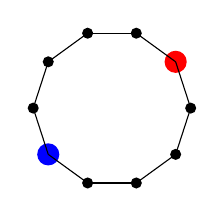
\begin{tikzpicture}
    % Draw the decagon
    \foreach \i in {1,...,10} {
            \coordinate (P\i) at ({cos(360/10*\i)}, {sin(360/10*\i)});
            \fill[black] (P\i) circle (2pt);
        }
    % Highlight two vertices
    \fill[red] (P1) circle (4pt); % First vertex
    \fill[blue] (P6) circle (4pt); % Second vertex
    % Draw the edges
    \foreach \i [evaluate=\i as \j using {mod(\i,10)+1}] in {1,...,10} {
            \draw (P\i) -- (P\j);
        }
\end{tikzpicture}
\hfill
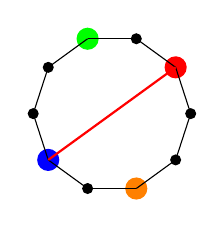
\begin{tikzpicture}
    % Draw the decagon
    \foreach \i in {1,...,10} {
            \coordinate (P\i) at ({cos(360/10*\i)}, {sin(360/10*\i)});
            \fill[black] (P\i) circle (2pt);
        }
    % Highlight four vertices
    \fill[red] (P1) circle (4pt); % First vertex
    \fill[blue] (P6) circle (4pt); % Second vertex
    \fill[green] (P3) circle (4pt); % Third vertex
    \fill[orange] (P8) circle (4pt); % Fourth vertex
    % Draw the edges
    \foreach \i [evaluate=\i as \j using {mod(\i,10)+1}] in {1,...,10} {
            \draw (P\i) -- (P\j);
        }
    % Draw the diagonals
    \draw[thick, red] (P1) -- (P6); % First diagonal
\end{tikzpicture}
\hfill
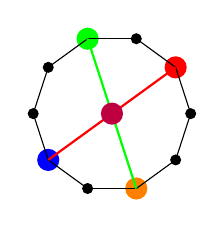
\begin{tikzpicture}
    % Draw the decagon
    \foreach \i in {1,...,10} {
            \coordinate (P\i) at ({cos(360/10*\i)}, {sin(360/10*\i)});
            \fill[black] (P\i) circle (2pt);
        }
    % Highlight four vertices
    \fill[red] (P1) circle (4pt); % First vertex
    \fill[blue] (P6) circle (4pt); % Second vertex
    \fill[green] (P3) circle (4pt); % Third vertex
    \fill[orange] (P8) circle (4pt); % Fourth vertex
    % Draw the edges
    \foreach \i [evaluate=\i as \j using {mod(\i,10)+1}] in {1,...,10} {
            \draw (P\i) -- (P\j);
        }
    % Draw the diagonals
    \draw[thick, red] (P1) -- (P6); % First diagonal
    \draw[thick, green] (P3) -- (P8); % Second diagonal
    % Highlight the intersection point
    \coordinate (Intersection) at (intersection of P1--P6 and P3--P8);
    \fill[purple] (Intersection) circle (4pt); % Intersection point
\end{tikzpicture}
\hfill
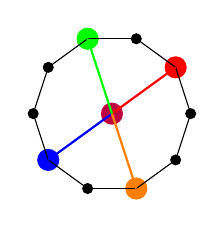
\begin{tikzpicture}
    % Draw the decagon
    \foreach \i in {1,...,10} {
            \coordinate (P\i) at ({cos(360/10*\i)}, {sin(360/10*\i)});
            \fill[black] (P\i) circle (2pt);
        }
    % Highlight four vertices
    \fill[red] (P1) circle (4pt); % First vertex
    \fill[blue] (P6) circle (4pt); % Second vertex
    \fill[green] (P3) circle (4pt); % Third vertex
    \fill[orange] (P8) circle (4pt); % Fourth vertex
    % Draw the edges
    \foreach \i [evaluate=\i as \j using {mod(\i,10)+1}] in {1,...,10} {
            \draw (P\i) -- (P\j);
        }
    % Calculate the intersection point
    \coordinate (Intersection) at (intersection of P1--P6 and P3--P8);
    \fill[purple] (Intersection) circle (4pt); % Intersection point

    % Draw the segmented diagonals
    \draw[thick, red] (P1) -- (Intersection); % Red part
    \draw[thick, blue] (Intersection) -- (P6); % Blue part
    \draw[thick, green] (P3) -- (Intersection); % Green part
    \draw[thick, orange] (Intersection) -- (P8); % Orange part
\end{tikzpicture}


Once this is done, we can note that of the existing diagonals, each intersection doubles the number of line segements. Illustrated in the figure above, we can see the existence of the green and red diagonals, but, the purple intersection splits them into 4 diagonal line segments, namely green, red, blue and orange.

So, the total number of diagonal line segments is
\begin{align*}
    \text{Total number of line segments} =
    \underbrace{\text{Number of pairs}- 10}_{\text{Exclude Sides}} + 2 \times \text{Number of intersections}. \\
\end{align*}
\mbox{\(\therefore \)} we get,
\begin{equation*}
    \Comb{10}{2} - 10 + 2 \times \Comb{10}{4} \text{ line segments}
\end{equation*}
\end{exampletcb}
